\documentclass[12pt,letterpaper]{exam}
\usepackage[lmargin=1in,rmargin=1in,tmargin=1in,bmargin=1in]{geometry}
\usepackage{../style/exams}

% -------------------
% Course & Exam Information
% -------------------
\newcommand{\course}{MAT 101: Exam 2}
\newcommand{\term}{Fall -- 2022}
\newcommand{\examdate}{11/21/2022}
\newcommand{\timelimit}{85 Minutes}

\setbool{hideans}{false} % Student: True; Instructor: False

% -------------------
% Content
% -------------------
\begin{document}

\examtitle
\instructions{Write your name on the appropriate line on the exam cover sheet. This exam contains \numpages\ pages (including this cover page) and \numquestions\ questions. Check that you have every page of the exam. Answer the questions in the spaces provided on the question sheets. Be sure to answer every part of each question and show all your work.} 
\scores
%\bottomline
\newpage

% ---------
% Questions
% ---------
\begin{questions}

% Question 1
\newpage
\question[10] As accurately as possible, plot the line $x= -\frac{5}{3}$ on the graph below.
	\[
	\fbox{
	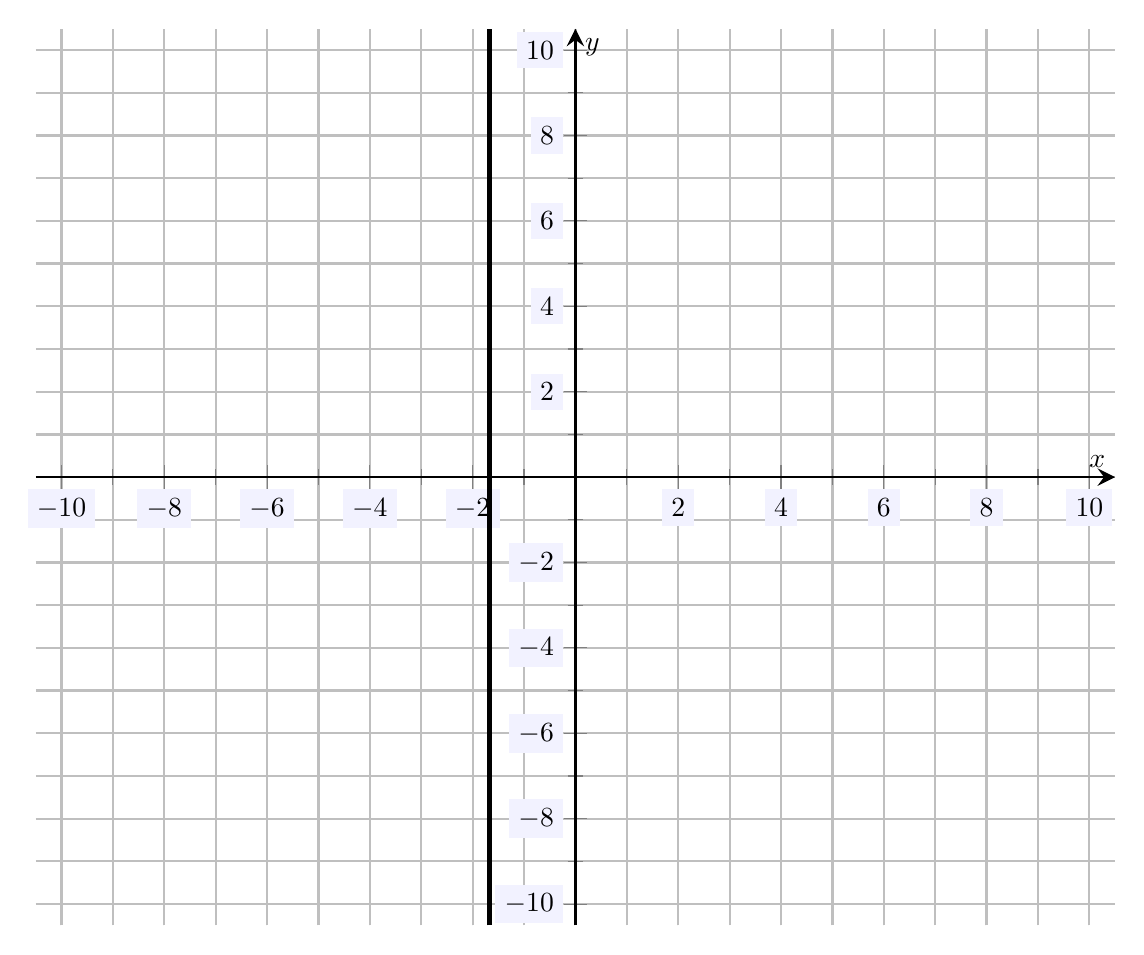
\begin{tikzpicture}[scale=2,every node/.style={scale=0.5}]
	\begin{axis}[
	grid=both,
	axis lines=middle,
	ticklabel style={fill=blue!5!white},
	xmin= -10.5, xmax=10.5,
	ymin= -10.5, ymax=10.5,
	xtick={-10,-8,-6,-4,-2,0,2,4,6,8,10},
	ytick={-10,-8,-6,-4,-2,0,2,4,6,8,10},
	minor tick = {-10,-9,...,10},
	xlabel=\(x\),ylabel=\(y\),
	]
	\draw[line width= 0.03cm] (-5/3,-10.5) -- (-5/3,10.5);
	\end{axis}
	\end{tikzpicture}
	}
	\] \pspace

{\itshape This is a vertical line located at $x= -\frac{5}{3}$.}



% Question 2
\newpage
\question[10] As accurately as possible, plot the line $y= \frac{3}{2}\, x - 3$ on the graph below. 
	\[
	\fbox{
	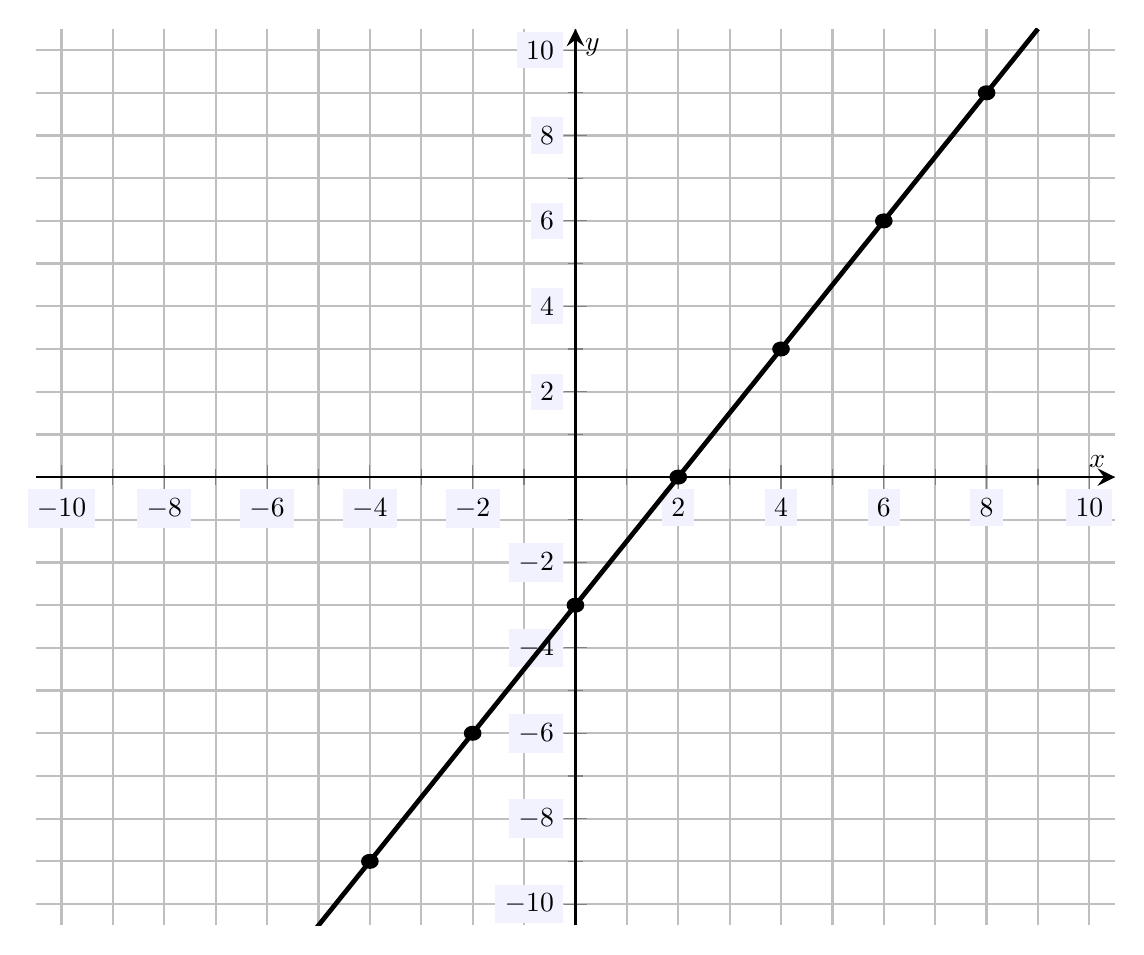
\begin{tikzpicture}[scale=2,every node/.style={scale=0.5}]
	\begin{axis}[
	grid=both,
	axis lines=middle,
	ticklabel style={fill=blue!5!white},
	xmin= -10.5, xmax=10.5,
	ymin= -10.5, ymax=10.5,
	xtick={-10,-8,-6,-4,-2,0,2,4,6,8,10},
	ytick={-10,-8,-6,-4,-2,0,2,4,6,8,10},
	minor tick = {-10,-9,...,10},
	xlabel=\(x\),ylabel=\(y\),
	]
	\addplot[domain=-6:9,samples=2,line width=0.03cm] (x, 3/2*x-3);
	\draw[fill=black] (-4,-9) circle (0.15);
	\draw[fill=black] (-2,-6) circle (0.15);
	\draw[fill=black] (0,-3) circle (0.15);
	\draw[fill=black] (2,0) circle (0.15);
	\draw[fill=black] (4,3) circle (0.15);
	\draw[fill=black] (6,6) circle (0.15);
	\draw[fill=black] (8,9) circle (0.15);
	\end{axis}
	\end{tikzpicture}
	}
	\] \pspace

{\itshape The line $y= \frac{3}{2}\,x - 3$ has $y$-intercept $(0, -3)$. The slope of the line is $m= \frac{3}{2}$. Interpreting $m= \frac{3}{2}$ as $\frac{\Delta y}{\Delta x}$, we see that for each increase of 2 in $x$, there is a corresponding increase of 3 in $y$. Alternatively, writing $m= \frac{3}{2}= \frac{-3}{-2}$ and interpreting this as $\frac{\Delta y}{\Delta x}$, we see that for each decrease of 2 in $x$, there is a decrease of 3 in $y$. Using the $y$-intercept and these interpretations of the slope to sketch points on the line (shown above), we obtain the sketch of the line.}



% Question 3
\newpage
\question[10] As accurately as possible, plot the line $5x + 4y= 10$ on the graph below. 
	\[
	\fbox{
	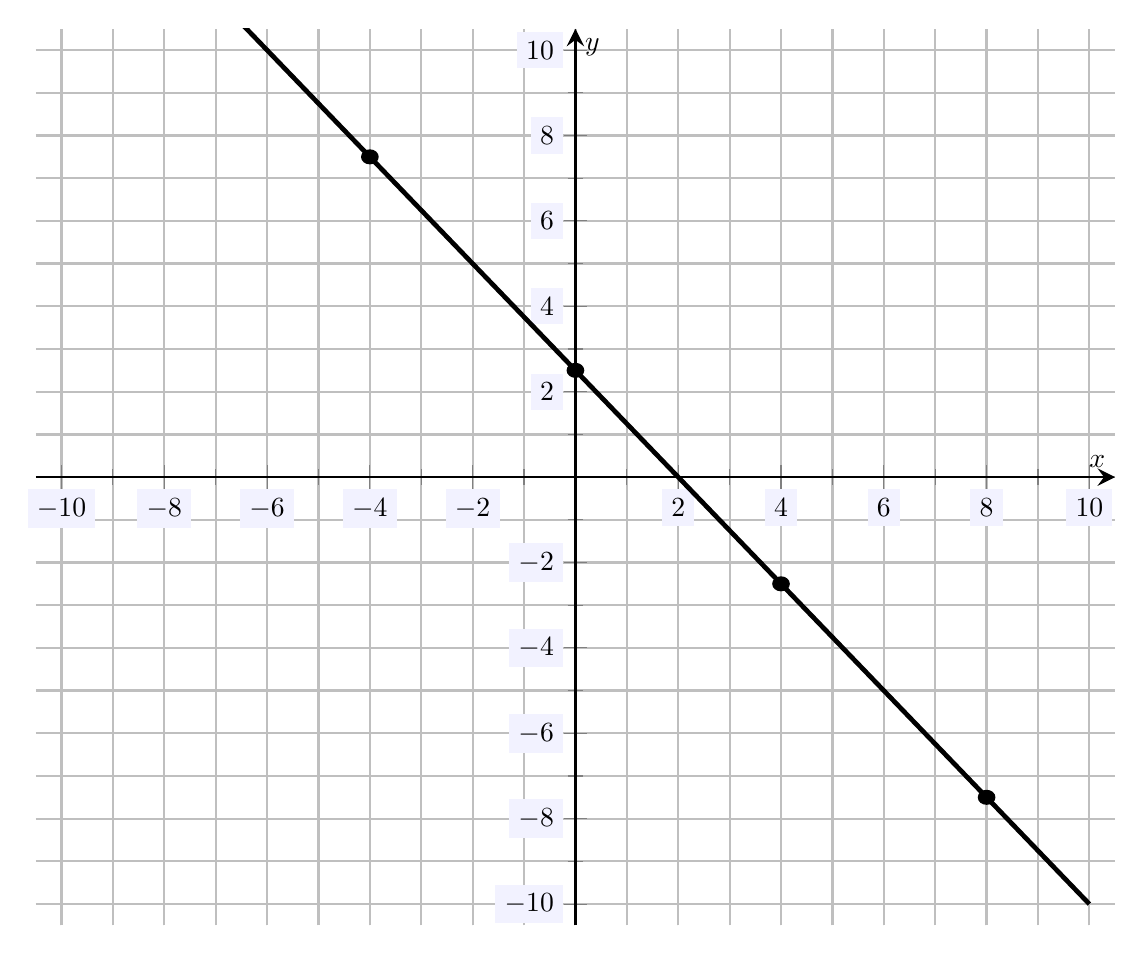
\begin{tikzpicture}[scale=2,every node/.style={scale=0.5}]
	\begin{axis}[
	grid=both,
	axis lines=middle,
	ticklabel style={fill=blue!5!white},
	xmin= -10.5, xmax=10.5,
	ymin= -10.5, ymax=10.5,
	xtick={-10,-8,-6,-4,-2,0,2,4,6,8,10},
	ytick={-10,-8,-6,-4,-2,0,2,4,6,8,10},
	minor tick = {-10,-9,...,10},
	xlabel=\(x\),ylabel=\(y\),
	]
	\addplot[domain=-10:10,samples=2,line width= 0.03cm] (x,-5/4*x+5/2);
	\draw[fill=black] (-8,25/2) circle (0.15);
	\draw[fill=black] (-4,15/2) circle (0.15);
	\draw[fill=black] (0,5/2) circle (0.15);
	\draw[fill=black] (4,-5/2) circle (0.15);
	\draw[fill=black] (8,-15/2) circle (0.15);
	\end{axis}
	\end{tikzpicture}
	}
	\] 

{\itshape First, observe that we have\dots
	\[
	\begin{aligned}
	5x &+ 4y= 10 \\
	4y&= -5x + 10 \\
	y&= -\frac{5}{4}\,x + \frac{10}{4} \\
	y&= -\frac{5}{4}\,x + \frac{5}{2}
	\end{aligned}
	\]
The line $y= -\frac{5}{4}\,x - 3$ has $y$-intercept $\big(0, \frac{5}{2} \big)$. The slope of the line is $m= -\frac{5}{4}= \frac{-5}{4}$. Interpreting $m= \frac{-5}{4}$ as $\frac{\Delta y}{\Delta x}$, we see that for each increase of 4 in $x$, there is a corresponding decrease of 5 in $y$. Alternatively, writing $m= -\frac{5}{4}= \frac{5}{-4}$ and interpreting this as $\frac{\Delta y}{\Delta x}$, we see that for each decrease of 4 in $x$, there is an increase of 5 in $y$. Using the $y$-intercept and these interpretations of the slope to sketch points on the line (shown above), we obtain the sketch of the line. \pspace

Alternatively, considering $5x + 4y= 10$, if $y= 0$, we have $5x= 10$, so that $x= 2$. But then $(2, 0)$ is a point on the line. If $x= 0$, we have $4y= 10$, so that $y= \frac{10}{4}= \frac{5}{2}$. But then $\big(0, \frac{5}{2} \big)$ is on the line. Connecting these points via a straight line, we have the line shown above. 
}



% Question 4
\newpage
\question[10] Consider the line given by $5x - 4y= 7$.
	\begin{enumerate}[(a)]
	\item Showing all your work and without referencing a graph, determine if $(-3, -2)$ is on the line. 
	\item Showing all your work and without referencing a graph, determine if $\big(1, -\frac{1}{2} \big)$ is on the line. 
	\end{enumerate} \pspace

\sol 
\begin{enumerate}[(a)]
\item We have\dots
	\[
	\begin{aligned}
	5x - 4y&= 7 \\
	5(-3) - 4(-2)&\stackrel{?}{=} 7 \\
	-15 + 8&\stackrel{?}{=} 7 \\
	-7&\neq 7 \\
	&\;\text{\xmark}
	\end{aligned}
	\] \pspace

\item We have\dots
	\[
	\begin{aligned}
	5x - 4y&= 7 \\
	5(1) - 4 \left(-\frac{1}{2} \right)&\stackrel{?}{=} 7 \\
	5 + 2&\stackrel{?}{=} 7 \\
	7&= 7 \\
	&\;\text{\cmark}
	\end{aligned}
	\]   
\end{enumerate}



% Question 5
\newpage
\question[10] Showing all your work and being sure to list the points, find at least three distinct points on the line $-7x + 3y= 10$. \pspace

\sol {\itshape To find points on the line, we can simple plug-in any value for $x, y$ and solve for the other. For instance, if\dots \pspace

$x= 0$: 
	\[
	\begin{aligned}
	-7x + 3y&= 10 \\
	0 + 3y&= 10 \\
	3y&= 10 \\
	y&= \frac{10}{3}
	\end{aligned}
	\]
Therefore, $\big(0, \frac{10}{3} \big)$ is on the line. \pspace

$y= 0$: 
	\[
	\begin{aligned}
	-7x + 3y&= 10 \\
	-7x + 0&= 10 \\
	-7x&= 10 \\
	x&= -\frac{10}{7}
	\end{aligned}
	\]
Therefore, $\big( -\frac{10}{7}, 0 \big)$ is on the line. \pspace

$x= 1$: 
	\[
	\begin{aligned}
	-7x + 3y&= 10 \\
	-7 + 3y&= 10 \\
	3y&= 17 \\
	y&= \frac{17}{3}
	\end{aligned}
	\]
Therefore, $\big(1, \frac{17}{3} \big)$ is on the line. \pspace

$y= 1$: 
	\[
	\begin{aligned}
	-7x + 3y&= 10 \\
	-7x + 3&= 10 \\
	-7x&= 7 \\
	x&= -1
	\end{aligned}
	\]
Therefore, $(-1, 1)$ is on the line. }



% Question 6
\newpage
\question[10] Consider the linear function $f(x)= 7 - \frac{6}{5}\,x$. Showing all your work, answer the following:
	\begin{enumerate}[(a)]
	\item Find the rate of change of $f(x)$.
	\item Interpret the rate of change of $f(x)$. 
	\item Determine whether $f(x)$ is an increasing or decreasing function.
	\item Determine the $y$-intercept of $f(x)$.
	\item Find the exact value of $f \big( \frac{2}{3} \big)$. 
	\end{enumerate} \pspace

\sol {\itshape
\begin{enumerate}[(a)]
\item The rate of change of $f(x)$ is the slope. Because $f(x)$ has the form $y= mx + b$, we see that the slope of $f(x)$ is $m= -\frac{6}{5}$. \pspace

\item We have $m= -\frac{6}{5}$. Writing $m= -\frac{6}{5}= \frac{-6}{5}$ and interpreting this as $\frac{\Delta y}{\Delta x}$, we see that each increase of 5 in $x$ results in a decrease of 6 in $y$. Alternatively, writing $m= -\frac{6}{5}= \frac{6}{-5}$ and interpreting this as $\frac{\Delta y}{\Delta x}$, we see that each decrease of 5 in $x$ results in an increase of 6 in $y$. \pspace

\item Because $m= -\frac{6}{5} < 0$, we see that $f(x)$ is decreasing. \pspace

\item Because $f(x)= 7 - \frac{6}{5}\,x$ has the form $y= mx + b$, we see that the $y$-intercept is $(0, 7)$. \pspace

\item We have\dots
	\[
	f \big( \frac{2}{3} \big)= 7 - \frac{6}{5} \cdot \frac{2}{3}= 7 - \frac{2}{5} \cdot \frac{2}{1}= 7 - \frac{4}{5}= \frac{35}{5} - \frac{4}{5}= \frac{31}{5}
	\]
\end{enumerate}
}



% Question 7
\newpage
\question[10] Consider the linear function $f(x)= -3(2x - 7)$. Showing all your work, answer the following:
	\begin{enumerate}[(a)]
	\item Find the rate of change of $f(x)$.
	\item Interpret the rate of change of $f(x)$. 
	\item Determine whether $f(x)$ is an increasing or decreasing function.
	\item Determine the $x$-intercept of $f(x)$.
	\item Find an $x$-value such that $f(x)= 9$.
	\end{enumerate} \pspace

\sol {\itshape First, we write $f(x)= -3(2x - 7)= -6x + 21$. 
\begin{enumerate}[(a)]
\item The rate of change of $f(x)$ is the slope. Because $f(x)= -6x + 21$ has the form $y= mx + b$, we see that the slope of $f(x)$ is $m= -6$. \pspace

\item We have $m= -6$. Writing $m= -6= \frac{-6}{1}$ and interpreting this as $\frac{\Delta y}{\Delta x}$, we see that each increase of 1 in $x$ results in a decrease of 6 in $y$. Alternatively, writing $m= -6= -\frac{6}{1}= \frac{6}{-1}$ and interpreting this as $\frac{\Delta y}{\Delta x}$, we see that each decrease of 1 in $x$ results in an increase of 6 in $y$. \pspace

\item Because $m= -6 < 0$, we see that $f(x)$ is decreasing. \pspace

\item Because $f(x)= -6x + 21$ has the form $y= mx + b$, we see that the $y$-intercept is $(0, 21)$. \pspace

\item If $f(x)= 9$, we have\dots
	\[
	\begin{aligned}
	f(x)&= 9 \\
	-6x + 21&= 9 \\
	-6x&= -12 \\
	x&= 2
	\end{aligned}
	\]
We can check: $f(2)= -6(2) + 21= -12 + 21= 9$.
\end{enumerate}
}



% Question 8
\newpage
\question[10] Find the equation of the line parallel to the line $y= 6 - x$ that has $x$-intercept $-12$. \pspace

\sol {\itshape Because the line is parallel to $y= 6 - x$, the line has the form $y= mx + b$. Because the line is parallel to $y= 6 - x$, it must have the same slope. The slope of the line $y= 6 - x$ has slope $-1$; therefore, the line has slope $m= -1$. Because the line has $x$-intercept $-12$, we know that $(-12, 0)$ is on the line. But then we have\dots
	\[
	\begin{aligned}
	y&= mx + b \\[0.3cm]
	y&= -x + b \\[0.3cm]
	0&= -(-12) + b \\[0.3cm]
	0&= 12 + b \\[0.3cm]
	b&= -12
	\end{aligned}
	\]
Therefore, the line is $y= -x - 12$. 
}



% Question 9
\newpage
\question[10] Find the equation of the line perpendicular to the line $y= -\frac{\pi}{2}$ that contains the $x$-intercept of the line $-7x + 5y= -3$. \pspace

\sol {\itshape Because the line is perpendicular to $y= -\frac{\pi}{2}$, which is horizontal, our line must be vertical. Therefore, the line has the form $x= c$ for some $c$. The $x$-intercept of the line $-7x + 5y= -3$ occurs when $y= 0$. But then we have $-7x= -3$. But then $x= \frac{3}{7}$. Therefore, the line contains the point $\big(\frac{3}{7}, 0 \big)$. But then the line must be $x= \frac{3}{7}$.}



% Question 10
\newpage
\question[10] Find the equation of the line that contains the $y$-intercept of $y= \frac{7}{11}\,x - 5$ and the point of intersection of $y= 4 - 3x$ and $y= \frac{1}{2}\,x + 18$. \pspace

\sol {\itshape Because the line $y= \frac{7}{11}\,x - 5$ has the form $y= mx + b$, the its $y$-intercept is $(0, -5)$. We now find the point of intersection of $y= 4 - 3x$ and $y= \frac{1}{2}\,x + 18$:
	\[
	\begin{aligned}
	4 - 3x&= \frac{1}{2}\,x + 18 \\
	2(4 - 3x)&= 2 \left( \frac{1}{2}\,x + 18 \right) \\
	8 - 6x&= x + 36 \\
	8 - 7x&= 36 \\
	-7x&= 28 \\
	x&= -4
	\end{aligned}
	\]
Using this in the line $y= 4 - 3x$. We have $y= 4 - 3(-4)= 4 + 12= 16$. Therefore, the line contains the point $(-4, 16)$. Because the line contains the point $(0, -5)$ and $(-4, 16)$, we have\dots
	\[
	m= \dfrac{\Delta y}{\Delta x}= \dfrac{16 - (-5)}{-4 - 0}= \dfrac{16 + 5}{-4 - 0}= \dfrac{21}{-4}= -\frac{21}{4}
	\]
But the line contains $(0, -5)$, so that we have\dots
	\[
	\begin{aligned}
	y&= mx + b \\
	-5&= -\frac{21}{4} \cdot 0 + b \\
	-5&= 0 + b \\
	b&= -5
	\end{aligned}
	\]
Therefore, the line $y= -\frac{21}{4}\,x - 5$.
}



% Question 11
\newpage
\question[10] Showing all your work, find the solution to the following:
	\[
	2(x - 9)= \frac{x}{3} + 7
	\] \pspace

\sol {\itshape We have\dots \pspace
	\[
	\begin{aligned}
	2(x - 9)&= \frac{x}{3} + 7 \\[0.3cm]
	2x - 18&= \frac{x}{3} + 7 \\[0.3cm]
	3(2x - 18)&= 3 \left( \frac{x}{3} + 7 \right) \\[0.3cm]
	6x - 54&= x + 21 \\[0.3cm]
	5x - 54&= 21 \\[0.3cm]
	5x&= 75 \\[0.3cm]
	x&= 15
	\end{aligned}
	\]
}



% Question 12
\newpage
\question[10] Showing all your work, find the solution to the following:
	\[
	\dfrac{5x - 3}{1 - x}= 13
	\] \pspace

\sol {\itshape We have\dots \pspace
	\[
	\begin{aligned}
	\dfrac{5x - 3}{1 - x}&= 13 \\[0.3cm]
	5x - 3&= 13(1 - x) \\[0.3cm]
	5x - 3&= 13 - 13x \\[0.3cm]
	18x - 3&= 13 \\[0.3cm]
	18x&= 16 \\[0.3cm]
	x&= \frac{16}{18} \\[0.3cm]
	x&= \frac{8}{9}
	\end{aligned}
	\]
}



% Question 13
\newpage
\question[10] Without explicitly finding the intersection, explain why the following lines $y= 2(7 - 5x)$ and $y= 5x + 2$ intersect. Showing all your work, find the intersection of the lines. \pspace

\sol {\itshape The line $y= 2(7 - 5x)= 14 - 10x$ has some $m= -10$. The line $y= 5x + 2$ has slope 5. Because $-10 \neq 5$, the lines cannot be parallel. But because the lines are not parallel, the lines must intersect.}



% Question 14
\newpage
\question[10] Thai Tanic is a new restaurant chain that has been expanding across the Northwest. It is projected that next year, it will have \$800,000 in profits and the following year it will have \$1.2~million in profits. 
	\begin{enumerate}[(a)]
	\item Under what assumptions is a linear model to predict the growth rate of this business appropriate?
	\item Find a linear model for the profit of this company $t$ years from today. 
	\item Interpret the slope of your linear model in (b).
	\item Interpret the $y$-intercept of your linear model in (b), if possible. 
	\item How long until the company has a profit of \$5~million? 
	\end{enumerate}



% Question 15
\newpage
\question[10] Sia Gogh is driving down the highway at 65~mph. She has been driving for 2~hours. Sia determines her total distance traveled $t$~hours from now is approximately $D(t)= 65t + 130$. 
	\begin{enumerate}[(a)]
	\item Explain why her distance traveled is approximately linear.
	\item Interpret the slope of $D(t)$.
	\item Interpret the $y$-intercept of $D(t)$. 
	\item How far has she traveled after a total of 10~hours?
	\end{enumerate}


\end{questions}
\end{document}